%!TEX root = ../report.tex

\chapter{Experiments}

The implementation described in the previous chapter was used to perform two sets of experiments. This chapter will
provide details on the experimental setup and discuss the experiments' results.


%%%%%%%%%%%%%%%%%%%%%%%%%%%%%%%%%%%%%%%%%%%%%%%%%%%%%%%%%%%%%%%%%%%%%%%%%%%%%%%%
\section{Setup}

\picHereWidth{experimental_setup}{Experiment setup: the robot assumes the same pose before each grasp.}
{fig:experiment_setup}{0.7\textwidth}

During the experiments, before each grasp, the robot is moved to a predefined location (marked on the floor) facing the
dining table in the C069 laboratory as shown in figure \ref{fig:experiment_setup}. Two sets of experiments are performed
for the two pose estimation methods described in section \ref{sub:pose_estimation}, for the objects shown in figure
\ref{fig:objects}. As mentioned previously, the SSD model used for object detection is trained on the COCO dataset.
Since this does not match the RoboCup@Home objects completely, we allow less confident detections to prioritize
evaluating the pose estimation methods as a baseline for grasp planning approaches. For example, the salt box or the
noodle box can be detected either as a bottle or a cup, whereas the duct tape can be detected as a bowl.

\begin{figure}[h!]
    \centering
    \small
    \begin{subfigure}[b]{0.4\textwidth}
        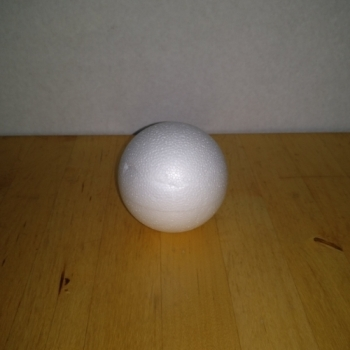
\includegraphics[width=\textwidth]{object_ball}
        \caption{A white styrofoam ball}
        \label{fig:object_ball}
    \end{subfigure}
    ~
    \begin{subfigure}[b]{0.4\textwidth}
        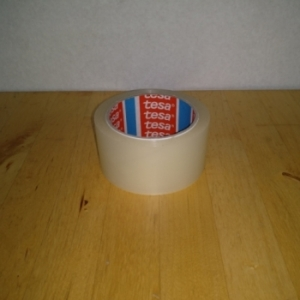
\includegraphics[width=\textwidth]{object_duct_tape}
        \caption{A roll of duct tape}
        \label{fig:object_duct_tape}
    \end{subfigure}

    \begin{subfigure}[b]{0.4\textwidth}
        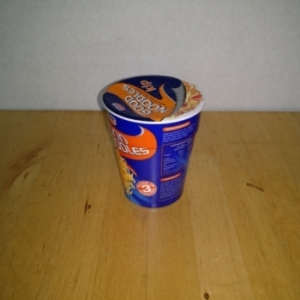
\includegraphics[width=\textwidth]{object_noodle_box}
        \caption{A cup noodles box}
        \label{fig:object_noodle_box}
    \end{subfigure}
    ~
    \begin{subfigure}[b]{0.4\textwidth}
        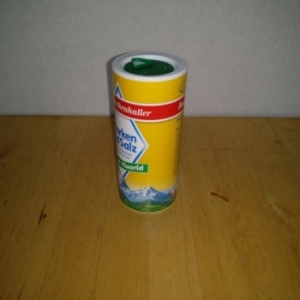
\includegraphics[width=\textwidth]{object_salt}
        \caption{A salt container}
        \label{fig:object_salt}
    \end{subfigure}
    \caption{Objects selected for the experiments.}\label{fig:objects}
\end{figure}

For both experiments, the robot first aligns itself with the estimated pose's $ y $-coordinate with respect to the
\texttt{base\_link} frame (shown in figure \ref{fig:base_link_frame}). The grasp is then executed using the learned
primitives, and the robot moves forward if the $ x $-coordinate is too far away. Also with respect to the
\texttt{base\_link} frame, objects detected more than 90cm away in the $ x $ direction and lower than the table height
of 75cm in the $ z $ direction are ignored. Objects' positions on the table are arbitrary for each grasp, but kept
within a 35cm distance from the table's edge to ensure reachability. The calculated $ x $ coordinate is offset by 4cm
to take into account the distance between the gripper coordinate frame and the fingertips. Pose detected further than
0.8m in the $ x $-axis or lower than 0.78m in the $ z $ axis are adjusted to these values to avoid severe collisions.
The robot arm still collides with the table using these adjusted coordinates. Only one object is grasped at a time.

For each object, the entire grasping pipeline is executed 20 times for 20 different positions. A trial is counted as
successful if the object stays in the gripper after the arm moves back close to the robot's body. If the object slips
off the gripper or the arm collides with the table, the execution is counted as a failure.


%%%%%%%%%%%%%%%%%%%%%%%%%%%%%%%%%%%%%%%%%%%%%%%%%%%%%%%%%%%%%%%%%%%%%%%%%%%%%%%%
\section{Results}

\begin{table}[h!]
    \small
    \begin{tabularx}{\textwidth}{L{0.2\textwidth}C{0.15\textwidth}C{0.15\textwidth}C{0.15\textwidth}C{0.15\textwidth}}
        \cmidrule[0.08em](){1-5}
        \multirow{2}{*}{Object} & \multicolumn{2}{c}{Mean $ x $} & \multicolumn{2}{c}{Minimum $ x $}    \\
        \cmidrule[0.08em](){2-5}
                                & Success   & Failure               & Success   & Failure               \\
        \cmidrule[0.08em](){1-5}
        Salt                    & 17        & 3                     & 16        & 4                     \\
        Ball                    & 8         & 12                    & 15        & 5                     \\
        Noodle box              & 16        & 4                     & 12        & 8                     \\
        Duct tape               & 7         & 13                    & 13        & 7                     \\
        \cmidrule[0.08em](){1-5}
    \end{tabularx}
    \caption{Results of the grasp experiments. On the left are results from using the mean $ x $ coordinates for
             estimating the grasp pose, and on the right are results from using the min coordinates along the
             $ x $-axis.}
    \label{table:grasp_exp_result}
\end{table}

Table \ref{table:grasp_exp_result} shows the grasp success/failure results of the experiments. During the experiments,
many of the failures while grasping the styrofoam ball is caused by the gripper pushing on the ball and making it roll
forward (an example is shown in figure \ref{fig:grasp_ball_fail}). For this object, grasping using the minimum
coordinate along the $ x $-axis proves to be much more reliable. Low objects like the roll of duct tape give low
estimates for the $ z $ coordinate, causing many failures via collisions between the arm and the table. This suggests
that a different approach vector from above may perform better for such objects. Many of the failures also occur
because of slipping while the arm is moving back, which suggests that verification from the force sensors may boost
grasp reliability.

\picHereWidth{grasp_ball_fail}{A failure instance where the gripper pushes on the ball and it rolls forward.}
             {fig:grasp_ball_fail}{\textwidth}
